\documentclass[11pt, a4paper, german]{article}
\usepackage[top=2cm, bottom=2cm]{geometry}
\pagestyle{plain}

\usepackage[german]{babel}
\usepackage{amsmath}
\usepackage{amsthm}
\usepackage{amssymb}
\usepackage{tikz}
\usepackage[utf8]{inputenc}
\usepackage{caption}
\usepackage{subcaption}

\newcommand{\HRule}{\rule{\linewidth}{0.5mm}}
\setlength{\parindent}{0cm}

\begin{document}
\begin{titlepage}

\begin{center}


% Oberer Teil der Titelseite:

\textsc{\LARGE Projektgruppe Angewandte Softwaretechnologie}\\[1.5cm]

\textsc{\Large Sommersemester 2015}\\[0.5cm]

\HRule \\[0.4cm] { \huge \bfseries DLVC Taverne}\\[0.2cm]
{\large \bfseries Ein Handbuch}\\[0.4cm]

\HRule \\[1.5cm]

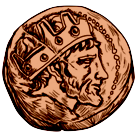
\includegraphics[width=0.6\textwidth]{./Logo3_1.png}\\[1cm]

\begin{minipage}{0.4\textwidth} \begin{flushleft} \large \emph{Author:}\\ Projektgruppe DLVC Taverne \end{flushleft} \end{minipage} \hfill \begin{minipage}{0.4\textwidth} \begin{flushright} \large \emph{Supervisor:} \\ Günther Kniesel \end{flushright} \end{minipage}

\vfill

{\large \today}

\end{center}

\end{titlepage}
\clearpage

\tableofcontents
\pagebreak

\section{Über das Programm}

\section{Das Hauptmenü}

\section{Der Charaktermanager}
\subsection{Der Gruppenmanager}
\subsection{Der Charaktermanager}
\subsection{Der Gegnermanager}

\section{Der Kampf}
\subsection{Die Gegnerrunde}
\subsection{Die Spielerrunde}
\subsection{Das Kampfende}

\section{Der Händler}
\subsection{Allgemein}
\subsection{Inventar}
\subsection{Rüstung und Waffen}

\section{Würfeln}

\end{document}